\documentclass[t]{beamer}
\usepackage{listings}
\usepackage{minted}

\usetheme{default}
\usebackgroundtemplate{
\includegraphics[width=\paperwidth]
                                       {../cpeb_bkground_topleftlogo.pdf}}

\setbeamertemplate{frametitle}{
  \centering\vspace{1mm}\insertframetitle\par\vspace{3mm}
}

\usepackage[style=nature,
            hyperref,
            backend=biber,
            isbn=false,
            doi=false,
            url=false,
            date=year,
            maxbibnames=3
           ]{biblatex}

\bibliography{kwip-phd.bib}

\title{\texttt{kWIP}: The k-mer Weighted Inner Product}
\author{Kevin Murray}
\institute{PhD Candidate, Borevitz Lab, CPEB, ANU}
\date{26 October 2015}

\usefonttheme{serif}

\begin{document}

{
\usebackgroundtemplate{
\includegraphics[width=\paperwidth]{../cpeb_bkground_centered.pdf}}
\begin{frame}
  \titlepage
  \vfill
\end{frame}
}

\begin{frame}{Overview}
  \begin{center}
    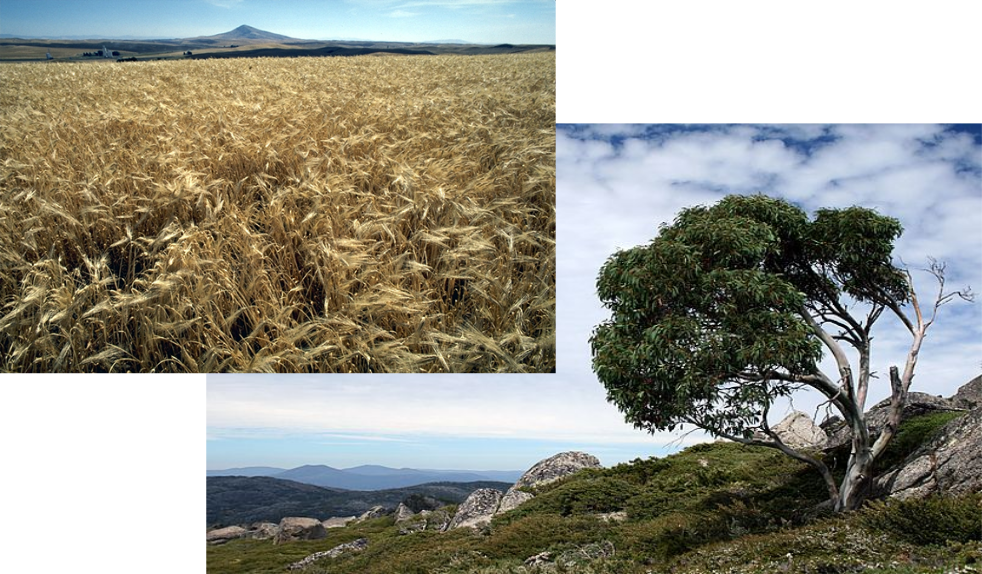
\includegraphics[width=\textwidth]{img/overview.png}
  \end{center}
\end{frame}

\begin{frame}{Large-scale population genomics}
  \begin{itemize}
    \item Moving from 100s to 1,000s or 10,000s of samples \textit{per PhD!}
      \pause
    \item Efficient algorithms to analyse large-scale genomic data
    \begin{itemize}
      \item Reference \& alignment free: \textit{less bias, de novo}
      \item Platform/protocol agnostic: \textit{future proof}
      \item Computationally efficient: \textit{not the bottleneck}
    \end{itemize}
  \end{itemize}
  \begin{center}
    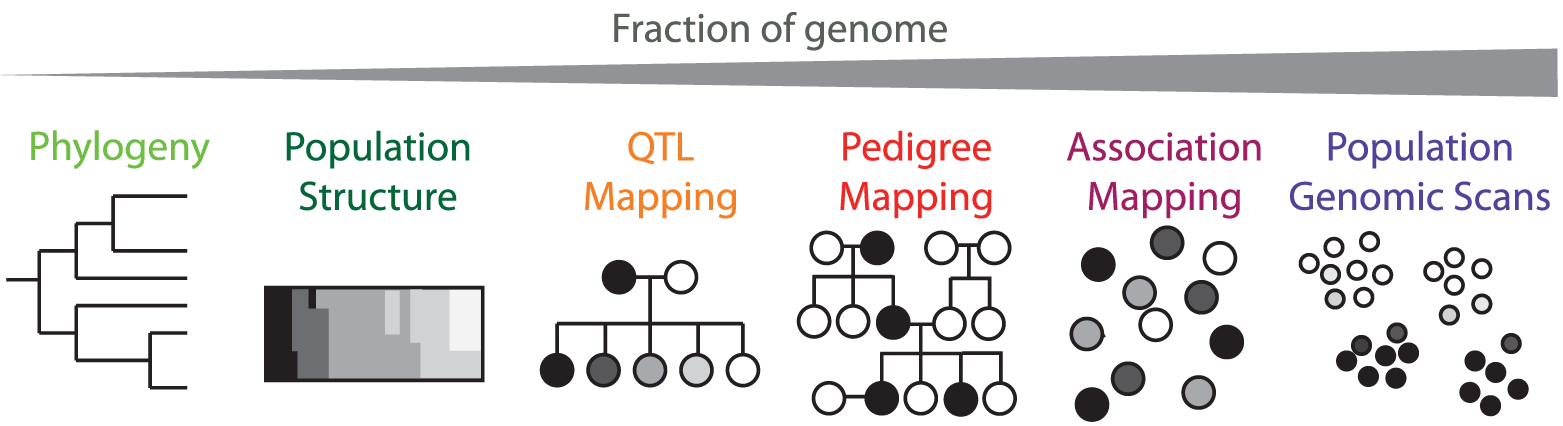
\includegraphics[width=\textwidth]{img/cross-scale.png}
  \end{center}
  \tiny{after \textcite{peterson_double_2012}}
\end{frame}

\begin{frame}{Presenting \texttt{kWIP}}
  \begin{itemize}
    \item $k$-mer based \textit{de novo} estimate of genetic similarity
    \item Produces a distance matrix from raw NGS reads
  \end{itemize}
  \begin{center}
    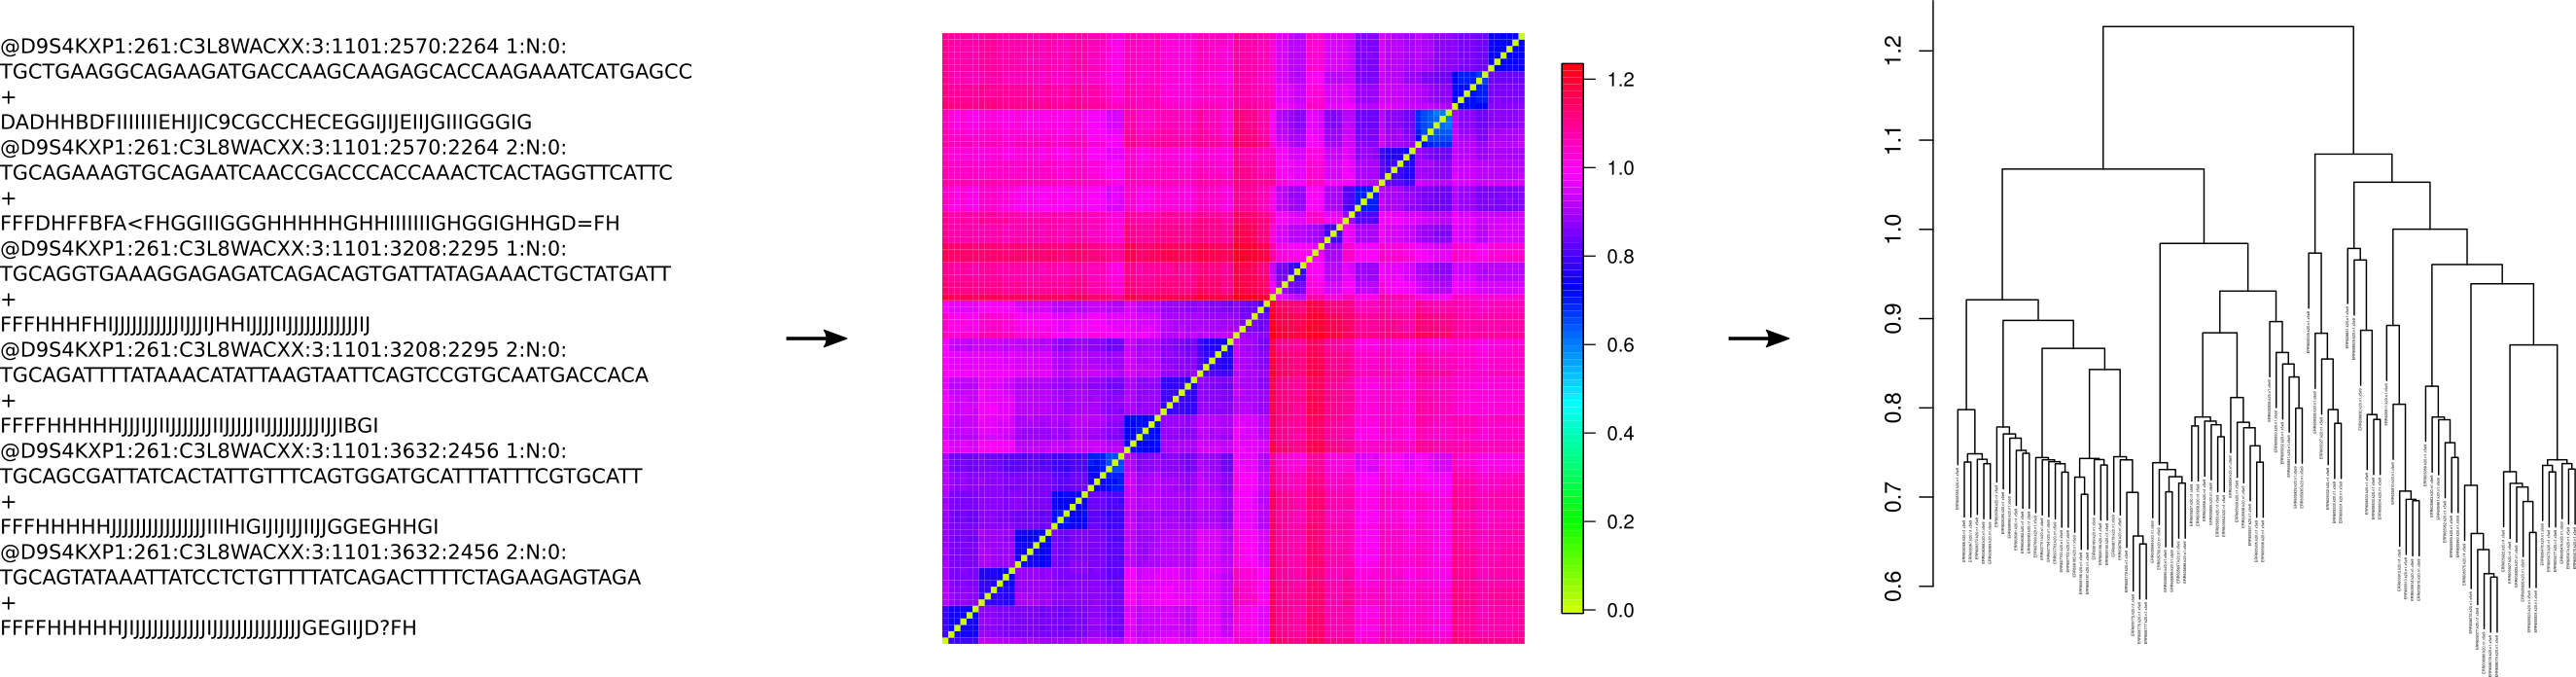
\includegraphics[width=\textwidth]{img/kwip-overview.png}
  \end{center}
\end{frame}

\begin{frame}{Why Estimate Similarity?}
  \begin{itemize}
    \item Rough approximation of sample relatedness required
      \begin{itemize}
        \item For natural collections
        \item As a technical control
      \end{itemize}
  \end{itemize}
  \pause
  \begin{center}
    \includegraphics<2>[width=\textwidth]{img/restruct-1}
    \includegraphics<3>[width=\textwidth]{img/restruct-2}
    \includegraphics<4>[width=\textwidth]{img/restruct-4}
    \begin{itemize}
      \item[]<2-4> \tiny{after \textcite{brachi_genome-wide_2011}}
    \end{itemize}
    \includegraphics<5>[width=\textwidth]{img/jared-tree.pdf}
    \includegraphics<6>[width=0.6\textwidth]{img/at80-tree.png}
  \end{center}
\end{frame}

\begin{frame}{Technological Overview}
  \begin{itemize}
    \item $k$-mer counting (bag-of-words)
    \begin{itemize}
      \item Decompose sequences to overlapping words of $k$
    \end{itemize}
    \pause
    \item Hashing and Probabilistic Data Structures
      \begin{itemize}
        \item Efficient storage \& compute of ``bag of words''
      \end{itemize}
    \pause
    \item (Weighted) Inner Products
      \begin{itemize}
        \item Similarity metric weighted by Shannon entropy
      \end{itemize}
  \end{itemize}
\end{frame}


\begin{frame}{\texttt{kWIP} Algorithm}
  \begin{itemize}
    \item For each run: count all $k$-mers into a Hash
    \item For each analysis:
      \begin{itemize}
        \item Calculate the entropy of population frequency ($H$)
        \item For each pair of runs $A$ and $B$, calculate \\
          $\sum\limits^{n}_{i=0} A_i \cdot B_i \cdot H_i$
      \end{itemize}
  \end{itemize}
  \begin{center}
    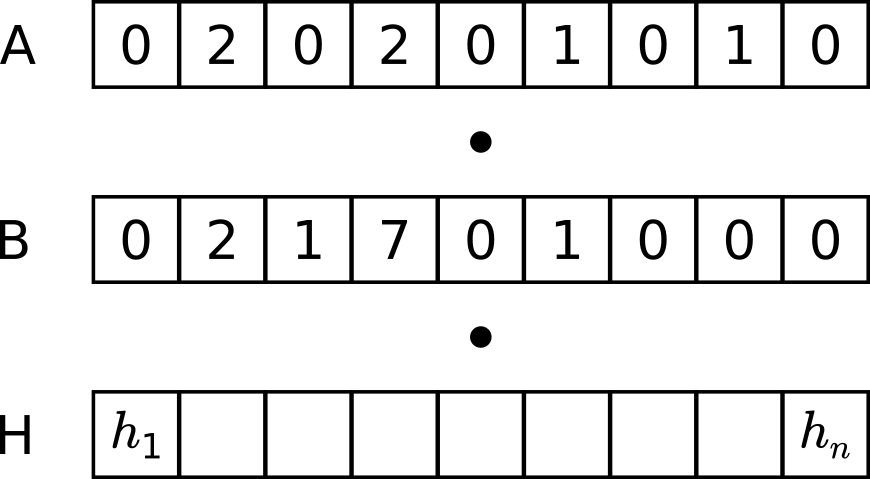
\includegraphics[width=0.4\textwidth]{img/hash-wip.png}
  \end{center}
\end{frame}


\begin{frame}{\texttt{kWIP}}
  \begin{itemize}
    \item The software:
      \begin{itemize}
        \item \texttt{C++}, $>$2000 lines of code
        \item Uses \texttt{khmer} for $k$-mer counting \& hashing
        \item Parallelised, fast
        \item GNU GPL licensed, source code on GitHub
      \end{itemize}
      \begin{center}
        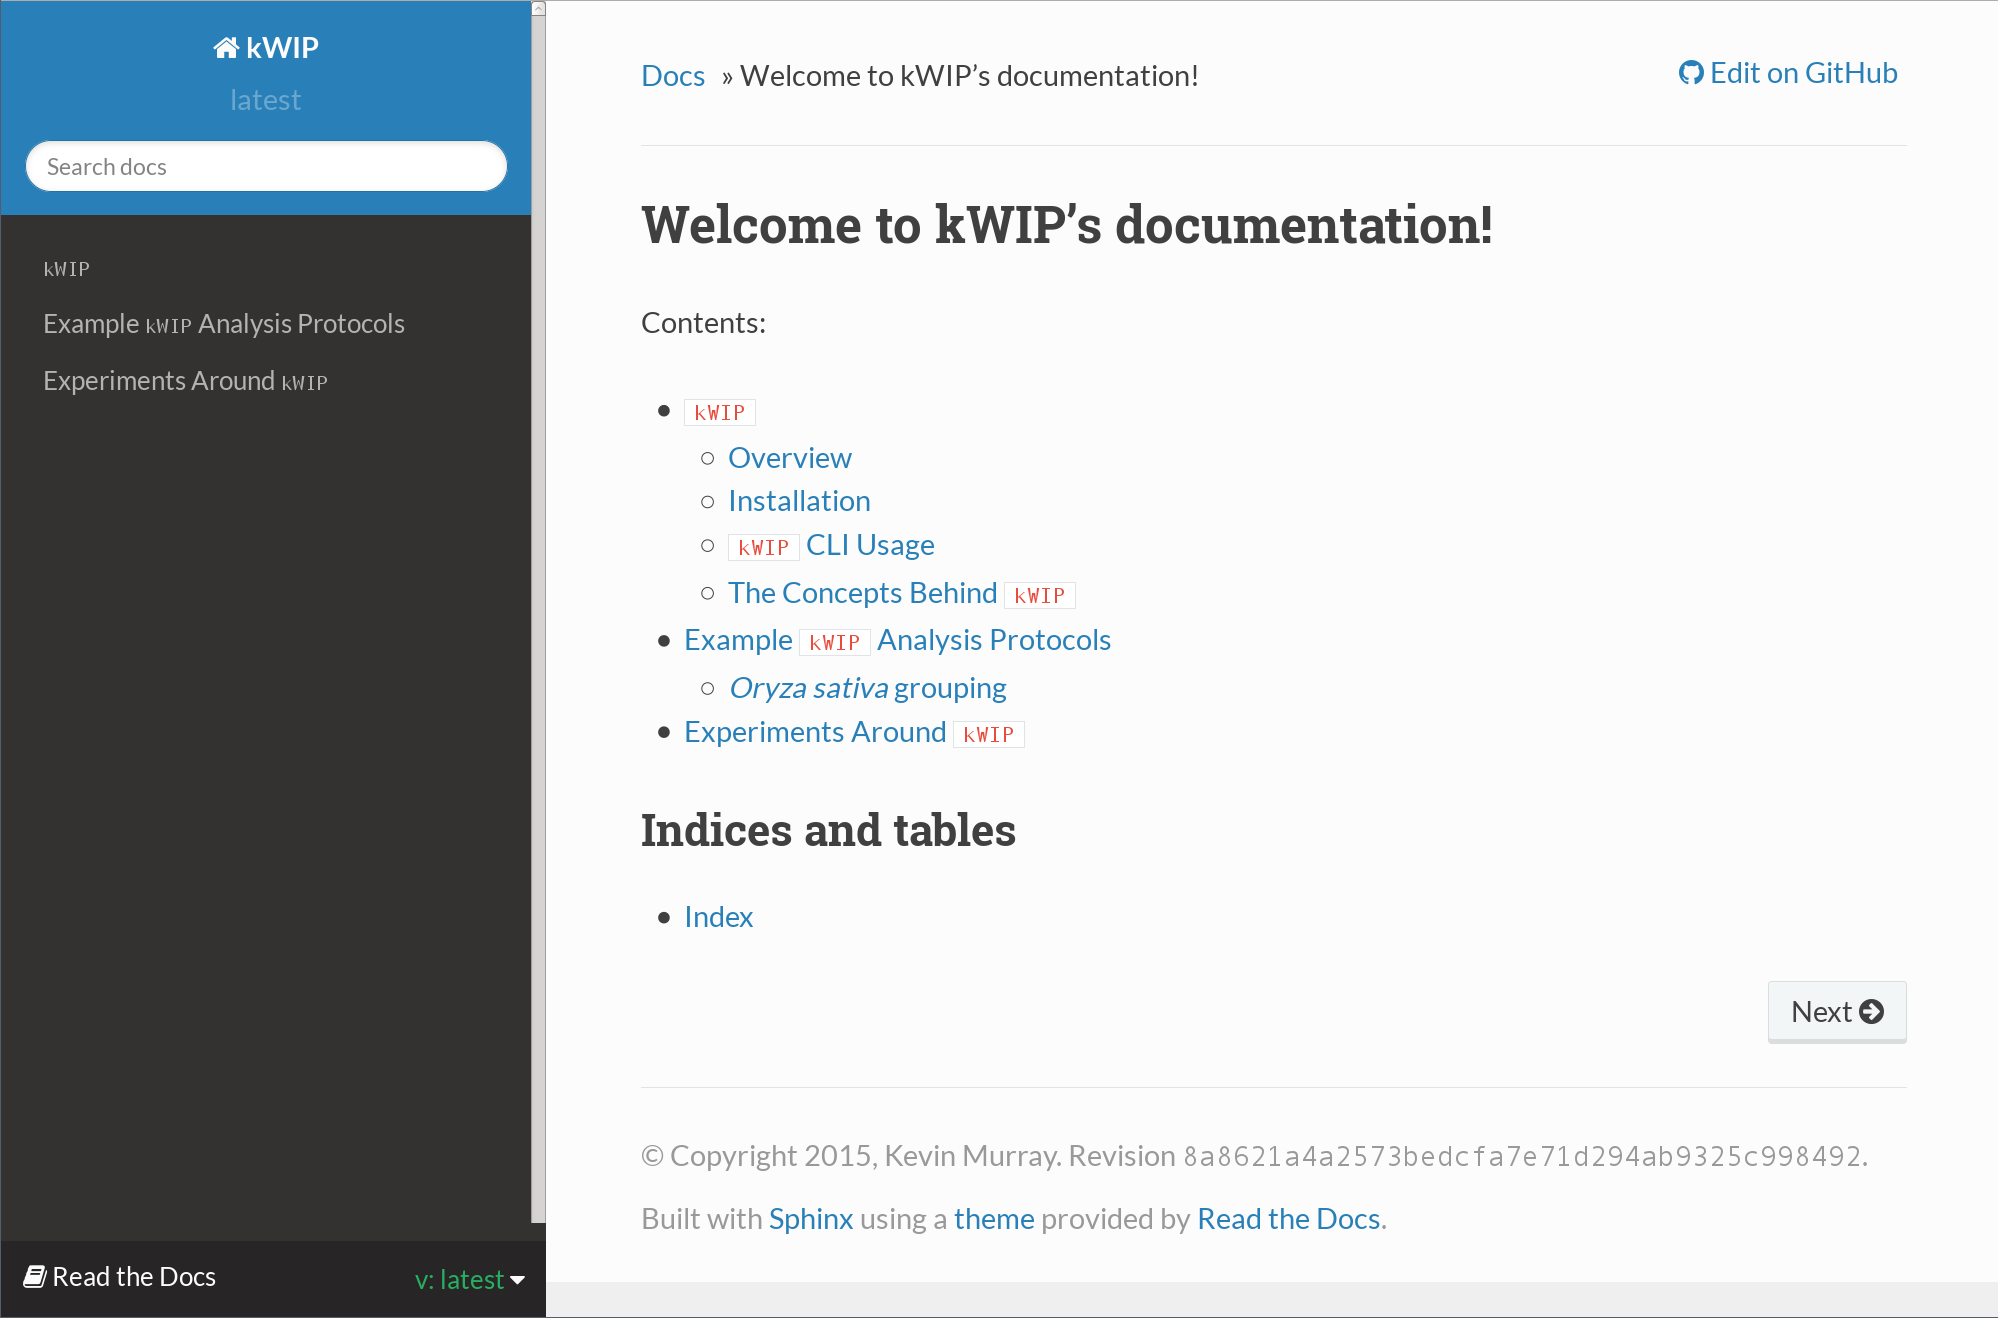
\includegraphics[width=0.5\textwidth]{img/kwip-doc-screenshot.png}
      \end{center}
  \end{itemize}
\end{frame}

\begin{frame}{Demonstration}
  \begin{itemize}
    \item Set of 96 rice runs from 16 samples (6 tech reps ea)
    \item Expectations:
      \begin{itemize}
        \item All runs cluster into groups of 6 reps (16 samples)
        \item Big split between Indica \& Japonica: (7 and 9 respectively here)
      \end{itemize}
    \item We see this with \texttt{kWIP}, not with Unweighted IP
    \item Took 8 hours on 16 CPU Raijin node, 60-80GB RAM
  \end{itemize}
\end{frame}

\begin{frame}
  \begin{center}
    \includegraphics<1>[width=0.6\textwidth]{img/dendro-wip.png}
    \includegraphics<2>[width=0.6\textwidth]{img/dendro-ip.png}
  \end{center}
\end{frame}

\begin{frame}{Conclusions}
  \begin{itemize}
    \item \texttt{kWIP} is implemented, $\beta$ software
    \item Estimates similarity reasonably well
    \item A few users in the audience (thanks!)
    \item Further simulations and experiments in progress
    \item Publication in preparation
  \end{itemize}
\end{frame}

\begin{frame}{Thanks}
  \begin{itemize}
    \item Supervisors: J Borevitz, S For\^et, G Huttley and B Pogson
    \item Christfried  Webers, Cheng Soon Ong, Norman Warthmann
    \item \texttt{khmer} folks: C. Titus Brown, Michael Crusoe, Camille Scott
          (DIB-lab) @ UC Davis
    \item Beta testers
    \item Yourselves
  \end{itemize}
\end{frame}

\begin{frame}[shrink=20]{References}
  \printbibliography
  \vfill
  .
\end{frame}

\end{document}
